%%%%%%%%%%%%%%%%%%%%%%%%%%%%%%%%%%%%%%
% Imports
%%%%%%%%%%%%%%%%%%%%%%%%%%%%%%%%%%%%%%
\documentclass[a4paper, 12pt]{article}
\usepackage[dutch]{babel}
\usepackage{CJK}
\usepackage[CJK, overlap]{ruby} %furigana support
\usepackage{float}
\usepackage{graphicx}
\usepackage{multirow}
\usepackage{pdflscape}
\usepackage[left=2cm,top=1cm,right=2cm,bottom=2cm, nohead,nofoot]{geometry}
\usepackage[usenames,dvipsnames]{color}
\usepackage{array}
\newcolumntype{s}{>{\centering\arraybackslash}m{1cm}}
\newcolumntype{B}{>{\centering\arraybackslash}m{4.0cm}}
\newcolumntype{L}{>{\centering\arraybackslash}m{7.0cm}}

%%%%%%%%%%%%%%%%%%%%%%%%%%%%%%%%%%%%%%
% Commands
%%%%%%%%%%%%%%%%%%%%%%%%%%%%%%%%%%%%%%
\renewcommand{\rubysize}{0.5}
\renewcommand{\rubysep}{-0.1ex}
\newcommand{\tran}[1]{{\itshape{\color{Gray}{#1}}}}

%%%%%%%%%%%%%%%%%%%%%%%%%%%%%%%%%%%%%%
% Start of document + settings
%%%%%%%%%%%%%%%%%%%%%%%%%%%%%%%%%%%%%%
\begin{document}
% Add support for japanese
%%\begin{CJK*}[dnp]{JIS}{min}
\begin{CJK*}{UTF8}{min}
\CJKtilde
%\CJKcaption{JIS}


%%%%%%%%%%%%%%%%%%%%%%%%%%%%%%%%%%%%%%
% Title page
%%%%%%%%%%%%%%%%%%%%%%%%%%%%%%%%%%%%%%
\title{Katori Technieken}
\author{Andy Nagels}
\maketitle
\thispagestyle{empty} %should remove the page number
%\pagestyle{empty} %should remove the page number in the whole document
\begin{figure}[H]
\centering
%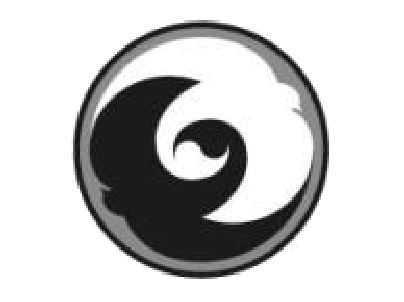
\includegraphics[width=2.5cm]{../img/schild_aikibudo.eps}
\end{figure}

\begin{center}
天真正伝香取神道流
\end{center}

\begin{figure}[H]
\centering
%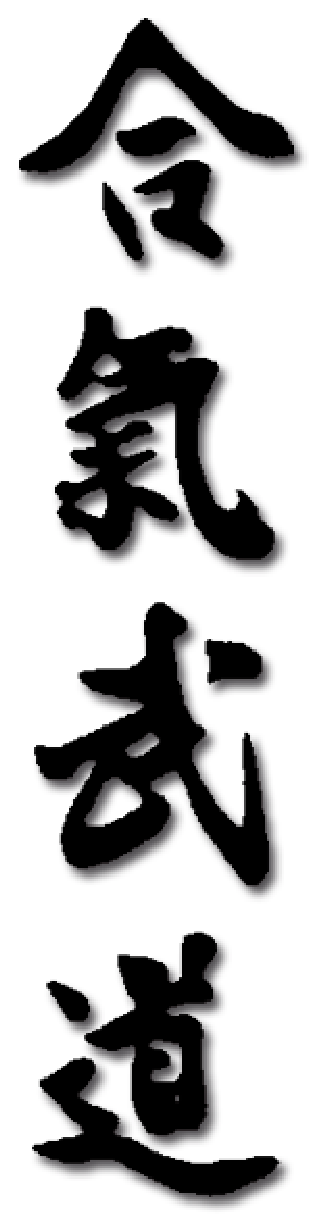
\includegraphics[width=1.0cm]{../img/aikibudo-kanji.eps}
\end{figure}


%%%%%%%%%%%%%%%%%%%%%%%%%%%%%%%%%%%%%%
% Disclaimer
%%%%%%%%%%%%%%%%%%%%%%%%%%%%%%%%%%%%%%
\newpage
\begin{center}
\textbf{Disclaimer}\\
De vertalingen in dit document zijn gemaakt door mezelf, m.b.v. offici\"{e}le documenten, moderne technologie en mijn eigen kennis van het Japans. Daar ik echter geen expert ben in de Japanse taal, is het mogelijk dat er fouten staan in dit document. Naarmate mijn kennis van Aikibudo en Japans stijgt, zal ik de nieuwe kennis die ik heb opgedaan dan ook gebruiken om dit document na te kijken en te corrigeren.\\
Dit document is dus niet als finaal te beschouwen. Het wordt reeds vrijgegeven omdat het kan helpen bij het onthouden van de technieken.
\end{center}
\begin{center}
\textit{{\em Opmerking:} De laatste versie kan gratis gedownload worden van de
volgende url: http://c.dommel.be/aikibudo.html.}
\end{center}


%%%%%%%%%%%%%%%%%%%%%%%%%%%%%%%%%%%%%%
% Table of contents
%%%%%%%%%%%%%%%%%%%%%%%%%%%%%%%%%%%%%%
\newpage
\setcounter{page}{1}
\pagenumbering{Roman}
\tableofcontents

%%%%%%%%%%%%%%%%%%%%%%%%%%%%%%%%%%%%%%
% General info
%%%%%%%%%%%%%%%%%%%%%%%%%%%%%%%%%%%%%%
\newpage
\setcounter{page}{1}
\pagenumbering{arabic}

\section{Inleiding}
\noindent Dit document bevat termen die gebruikt worden in aikibudo.

\section{De Japanse taal}
\noindent Alvorens we de berippen bekijken, dient een korte uitleg gegeven te worden over de Japanse taal.\\

\noindent Japans is opgebouwd uit 3 grote onderdelen: \textit{hiragana, katakana} en \textit{kanji}.\\

\noindent Hiragana en katakana zijn allebei een \textit{phonetisch} alfabet. Dat wil zeggen dat het symbolen voorstelt, die een klank uitbeelden.
Japans heeft dus geen aparte letters, zoals de meeste Westerse alfabetten.\\

\noindent \textbf{Hiragana} wordt gebruikt om zinnen te vormen en grammatica toe te passen op de Japanse taal. Het toont hoe Japans wordt uitgesproken.\\

\noindent \textbf{Katakana} bevat dezelfde klanken en enkele extra klanken. Het is ontstaan om de verschillende buitenlandse termen te kunnen uitspreken. Zo worden bvb. namen van niet Japanners in katakana geschreven.\\

\noindent \textbf{Kanji} zijn de meer complexe Japanse symbolen, die woorden en begrippen voorstellen. Ook Japanse namen en plaatsnamen worden meestal met kanji geschreven. Om te weten hoe deze symbolen worden uitgesproken, wordt gebruik gemaakt van hiragana, omdat hiragana een phonetisch alfabet is dat klanken in beeld brengt.\\

\noindent \textbf{Romaji} is een westerse schrijfwijze van Japanse klanken. Het wordt in Japan ook gebruikt om op een computer te typen.
Het is deze schrijfwijze, die het mogelijk maakt voor mensen die geen Japans kennen, om Japanse termen correct uit te spreken.

\noindent \textbf{Furigana} zijn kleine symbolen boven de kanji die in hiragana weergeven hoe de kanji moet worden uitgesproken.

\noindent In de tabel hieronder, kan je een overzicht vinden van de verschillende alfabetten, ter verduidelijking van bovenstaande uitleg.\\

\begin{table}[H]
\begin{center}
\begin{tabular}{c|c|c|c}
Nederlands alfabet & Hiragana & Katakana & Romaji\\
\hline
a &  あ & ア & a\\
k & bestaat niet & bestaat niet & bestaat niet\\
bestaat niet & か & カ & ka
\end{tabular}
\end{center}
\caption{Een kleine vergelijking ter verduidelijking}
\label{vergelijking_alfabetten}
\end{table}

\noindent De begrippen in dit document, zijn op volgende manier weergegeven:\\

\textit{Nederlandse omschrijving} $|$ \textit{Japanse term [met hiragana uitspraak boven de kanji]} $|$ \textit{romaji uitspraak}\\

\noindent De technieken zijn echter te lang om op die manier weer te geven. Zij staan dus onder elkaar:\\

\begin{center}
\textit{Nederlandse term}\\
\textit{Japanse term [met hiragana uitspraak boven de kanji]}\\
\textit{Romaji uitspraak}
\end{center}


\section{Uitspraak}
\noindent Een aantal letters worden iets anders uitgesproken in de romaji uitspraak, t.o.v. het Nederlands.
Het is interessant om dit even te lezen, om zo geen verkeerde uitspraak te leren voor de techniek.\\

\noindent j: $|zj|$ zoals in strand\textbf{j}anet, \textbf{J}efke, ... (en NIET zoals in \textbf{J}ommeke)\\
ch: $|tsj|$ zoals in \textbf{tsj}oeke \textbf{tsj}oeke tuut tuut\\
sh: $|sj|$ zoals in \textbf{ch}oco, \textbf{sh}ampoo, ...\\
u: korte $|oe|$ zoals in nen t\textbf{oe}k \textbf{oe}p aa bakkes, vake en m\textbf{oe}ke, ...\\
\={o} of ou: lange $|o|$ zoals in b\textbf{oo}t\\
\={u} of uu: lange $|u|$ zoals in v\textbf{uu}r


%%%%%%%%%%%%%%%%%%%%%%%%%%%%%%%%%%%%%%
% General terminology
%%%%%%%%%%%%%%%%%%%%%%%%%%%%%%%%%%%%%%
\section{Algemene terminologie}
\subsection{Algemeen}
\begin{table}[H]
\begin{center}
\begin{tabular}{c|c|c}
    \ruby{基本}{きほん} & kihon & \tran{basis/oorsprong/standaard}\\
    \hline
    \ruby{受身}{うけみ} & ukemi & \tran{de kunst van het veilig vallen}\\
    \hline
    \ruby{取}{と}り & tori & \tran{vastpakken}\\
    \hline
    \ruby{押}{お}さえ & osae & \tran{controle}\\
    \hline
    \ruby{技}{わざ} & waza & \tran{techniek}\\
    \hline
    \ruby{構}{かま}え & kamae & \tran{houding}
\end{tabular}
\end{center}
\end{table}

\subsection{Richtingen en gebieden}
\begin{table}[H]
\begin{center}
\begin{tabular}{c|c|c}
    \ruby{右}{みぎ} & migi & rechts\\
    \hline
    \ruby{左}{ひだり} & hidari & links\\
    \hline
    \ruby{後}{うし}ろ & ushiro & achterkant\\
    \hline
    \ruby{前}{まえ} & mae & voorkant\\
    \hline
    \ruby{上段}{じょうだん} & j\={o}dan & bovenste laag\\
    \hline
    \ruby{中段}{ちゅうだん} & ch\={u}dan & midden\\
    \hline
    \ruby{土}{ど} & do & grond
\end{tabular}
\end{center}
\end{table}

\subsection{Acties}
\begin{table}[H]
\begin{center}
\begin{tabular}{c|c|c}
    \ruby{投}{な}げ & nage & worp\\
    \hline
    \ruby{頭突}{ずつ}き & zutsuki & kopstoot\\
    \hline
    \ruby{蹴}{け}り & keri & trap\\
    \hline
    \ruby{絞殺}{こうさつ} & k\={o}satsu & wurging\\
    \hline
    \ruby{返}{がえ}し & gaeshi & omkering/terug sturen\\
    \hline
    \ruby{横蹴}{よこけ}り & yoko keri & zijwaartse trap\\
    \hline
    \ruby{突}{つ}き & tsuki & stoot
\end{tabular}
\end{center}
\end{table}

\subsection{Lichaamsdelen}
\begin{table}[H]
\begin{center}
\begin{tabular}{c|c|c}
    \ruby{体}{たい} & tai & lichaam\\
    \hline
    \ruby{手}{て} & te & hand\\
    \hline
    \ruby{肘}{ひじ} & hiji & elleboog/elleboogstoot\\
    \hline
    \ruby{膝}{ひざ} & hiza & knie\\
    \hline
    \ruby{手首}{てくび} & tekubi & pols\\
    \hline
    \ruby{小手}{こて} & kote & onderarm\\
    \hline
    \ruby{肩}{かた} & kata & schouder
\end{tabular}
\end{center}
\end{table}

\subsection{Andere begrippen}
\begin{table}[H]
\begin{center}
\begin{tabular}{c|c|c}
    \ruby{捻}{ねじ} & neji & draaien\\
    \hline
    \ruby{表}{おもて} & omote & uitwendig\\
    \hline
    \ruby{表}{ひょう} & hy\={o} & tabel\\
    \hline
    \ruby{型}{かた} & kata & standaard vorm van een beweging in de krijgskunst
\end{tabular}
\end{center}
\end{table}

\subsection{Leerstof}
\begin{table}[H]
\begin{center}
\begin{tabular}{c|c|c}
    \ruby{体捌}{たいさば}き & tai sabaki & lichaam hanteren\\
    \hline
    \ruby{受身}{うけみ}\ruby{技}{わざ} & ukemi waza & valtechnieken\\
    \hline
    \ruby{突}{つ}き\ruby{技}{わざ} & tsuki waza & stoottechnieken\\
    \hline
    \ruby{蹴}{け}り\ruby{技}{わざ} & keri waza & traptechnieken\\
    \hline
    \ruby{補}{ほ}\ruby{助}{じょ}\ruby{運}{うん}\ruby{動}{どう} & hojo und\={o} & hulp-oefening\\
    \hline
    \ruby{掴}{つか}み\ruby{型}{かた}と\ruby{手}{て}\ruby{解}{ほど}き & tsukami kata to te hodoki & grip kata en hand lossen\\
    \hline
    \ruby{追加}{ついか}の\ruby{技}{わざ} & tsuika no waza & aanvullende technieken\\
    \hline
    \ruby{基本}{きほん}\ruby{投}{な}げ\ruby{技}{わざ} & kihon nage waza & basis werp technieken\\
    \hline
    \ruby{基本}{きほん}\ruby{押}{お}さえ\ruby{技}{わざ} & kihon osae waza & basis controle technieken\\
    \hline
    \ruby{歴}{れき}\ruby{史}{し}\ruby{的}{てき}\ruby{技}{わざ} & reki shiteki  & historische technieken\\
    \hline
    \ruby{型}{かた} & kata & standaard vorm van een beweging in de krijgskunst\\
    \hline
    \ruby{和}{わ}の\ruby{精}{せい}\ruby{神}{しん} & wa no seishin & geest in harmonie\\ 
    \hline
    \ruby{防衛}{ぼうえい}の\ruby{棒}{ぼう} & b\={o}ei no b\={o} & verdedigingsstok\\
    \hline
    \ruby{乱取}{らんど}り & randori & vrij gevecht
\end{tabular}
\end{center}
\end{table}

\subsection{Gradaties}
\begin{table}[H]
\begin{center}
\begin{tabular}{c|c|c}
    \ruby{初}{しょう}\ruby{級}{きゅう} & sh\={o} ky\={u} & elementair niveau\\
    \hline
    \ruby{中}{ちゅう}\ruby{級}{きゅう} & ch\={u} ky\={u} & tussenliggend niveau\\
    \hline
    \ruby{上}{じょう}\ruby{級}{きゅう} & j\={o} ky\={u} & senior-niveau
\end{tabular}
\end{center}
\end{table}


%%%%%%%%%%%%%%%%%%%%%%%%%%%%%%%%%%%%%%
% Kyuu techniques
%%%%%%%%%%%%%%%%%%%%%%%%%%%%%%%%%%%%%%
\newpage
\section{級の技・Ky\={u} technieken}
\subsection{6de ky\={u} [SH\={O}KY\={U}]}
\subsubsection{体捌き・Tai sabaki}
\begin{table}[H]
\begin{center}
\begin{tabular}{cc}
    \ruby{入}{い}り\ruby{身}{み} & \ruby{大}{おお}\ruby{入}{い}り\ruby{身}{み} \\
    iri mi & \={o} iri mi\\
    inkomend lichaam & groot inkomend lichaam
\end{tabular}
\end{center}
\label{kyuu_6_taisabaki}
\end{table}

\subsubsection{受身技・Ukemi waza}
\begin{table}[H]
\begin{center}
\begin{tabular}{c}
    \ruby{後}{うし}ろ\\
    ushiro\\
    achterwaarts
\end{tabular}
\end{center}
\label{kyuu_6_ukemi_waza}
\end{table}

\subsubsection{突き技・Tsuki waza}
\begin{table}[H]
\begin{center}
\begin{tabular}{c}
    \ruby{直}{ちょく}\ruby{つ}{突}き\\
    choku tsuki\\
    rechte stoot 
\end{tabular}
\end{center}
\label{kyuu_6_tsuki_waza}
\end{table}

\subsubsection{蹴り技・Keri waza}
\begin{table}[H]
\begin{center}
\begin{tabular}{c}
    \ruby{前}{まえ}\ruby{蹴}{け}り\\
    mae keri\\
    voorwaartse trap
\end{tabular}
\end{center}
\label{kyuu_6_keri_waza}
\end{table}

\subsubsection{補助運動・Hojo und\={o}}
\begin{table}[H]
\begin{center}
\begin{tabular}{c}
    \ruby{}{}\ruby{}{}\\
    nigiri kaeshi\\
    ?\\
    \hline
    \ruby{}{}\\
    neji kaeshi\\
    ?
\end{tabular}
\end{center}
\label{kyuu_6_hojo_undou}
\end{table}

\subsubsection{掴み型と手解き・Tsukami kata \& te hodoki}
\begin{table}[H]
\begin{center}
\begin{tabular}{c}
    \ruby{}{}\ruby{}{}\\
    junte dori\\
    ?\\
    \hline
    \ruby{}{}\\
    dosoku te dori\\
    ?
\end{tabular}
\end{center}
\label{kyuu_6_te_hodoki}
\end{table}

\subsubsection{追加技・Aanvullende technieken}
\begin{table}[H]
\begin{center}
\begin{tabular}{c}
    \ruby{}{}\ruby{}{}\\
    ushiro kata otoshi\\
    ?
\end{tabular}
\end{center}
\label{kyuu_6_additional}
\end{table}

\subsubsection{基本投げ技・Kihon nage waza}
\begin{table}[H]
\begin{center}
\begin{tabular}{rl}
    \ruby{}{}\ruby{}{} & \\
    mukae daoshi & (ura yoko men uchi)\\
    ? & (?)
\end{tabular}
\end{center}
\label{kyuu_6_kihon_nage_waza}
\end{table}

\subsubsection{基本押え技・Kihon osae waza}
\begin{table}[H]
\begin{center}
\begin{tabular}{rl}
    \ruby{}{}\ruby{}{} & \\
    ushiro neji kudaki & (tsuki ch\={u}dan)\\
    ? & (?)
\end{tabular}
\end{center}
\label{kyuu_6_kihon_osae_waza}
\end{table}

\subsubsection{歴史的技・Historische technieken}
\begin{table}[H]
\begin{center}
\begin{tabular}{rl}
    \ruby{}{}\ruby{}{} & \\
    daito ryu aikijujutsu & ikkajo (idori)\\
    ? & ? (?)
\end{tabular}
\end{center}
\label{kyuu_6_historic}
\end{table}


\newpage
\subsection{5de ky\={u} [SH\={O}KY\={U}]}
\subsubsection{体捌き・Tai sabaki}
\begin{table}[H]
\begin{center}
\begin{tabular}{cc}
    ? & \ruby{大}{おお}? \\
    irimi & \={o} irimi\\
    ? & ? 
\end{tabular}
\end{center}
\label{kyuu_1_taisabaki}
\end{table}

\subsubsection{受身技・Ukemi waza}
\subsubsection{突き技・Tsuki waza}
\subsubsection{蹴り技・Keri waza}
\subsubsection{補助運動・Hojo undo}
\subsubsection{掴み型と手解き・Tsukami kata \& te hodoki}
\subsubsection{追加技・Aanvullende technieken}
\subsubsection{基本投げ技・Kihon nage waza}
\subsubsection{基本押え技・Kihon osae waza}
\subsubsection{歴史的・Historische technieken}


\newpage
\subsection{4de ky\={u} [CH\={U}KY\={U}]}
\subsubsection{体捌き・Tai sabaki}
\begin{table}[H]
\begin{center}
\begin{tabular}{rl}
    ? & (?)\\
    ? & (ichi ? ichi)\\
    esquives canalisation? &  
\end{tabular}
\end{center}
1 \leftrightarrow 1
\label{kyuu_4_taisabaki}
\end{table}
\begin{center}
    1 \leftrightarrow 1
\end{center}

\subsubsection{受身技・Ukemi waza}
\begin{table}[H]
\begin{center}
\begin{tabular}{c}
    \ruby{}{}\\
    yoko ukemi\\
    zijwaartse (rol? val?)
\end{tabular}
\end{center}
\label{kyuu_4_ukemi_waza}
\end{table}

\subsubsection{突き技・Tsuki waza}
\begin{table}[H]
\begin{center}
\begin{tabular}{c}
    \ruby{}{}\\
    gyaku tsuki\\
    ?\\
    \hline
    \ruby{}{}\\
    hineri uchi\\
    ?
\end{tabular}
\end{center}
\label{kyuu_4_tsuki_waza}
\end{table}

\subsubsection{蹴り技・Keri waza}
\begin{table}[H]
\begin{center}
\begin{tabular}{c}
    \ruby{}{}\ruby{蹴}{り}\\
    yoko keri\\
    zijwaartse trap
\end{tabular}
\end{center}
\label{kyuu_4_keri_waza}
\end{table}

\subsubsection{補助運動・Hojo undo}
\begin{table}[H]
\begin{center}
\begin{tabular}{c}
    \ruby{}{}\ruby{}{}\\
    shinogi\\
    (appel scheppen he :p)?
\end{tabular}
\end{center}
\label{kyuu_4_hojo_undo}
\end{table}

\subsubsection{掴み型と手解き・Tsukami kata \& te hodoki}
\begin{table}[H]
\begin{center}
\begin{tabular}{c}
    \ruby{}{}\ruby{}{}\\
    mae eri dori\\
    ?\\
    \hline
    \ruby{}{}\\
    sodee dori\\
    ?\\
    \hline
    \ruby{}{}\\
    ushiro ry\={o} te dori\\
    ?
\end{tabular}
\end{center}
\label{kyuu_4_te_hodoki}
\end{table}

\subsubsection{追加技・Aanvullende technieken}
\begin{table}[H]
\begin{center}
\begin{tabular}{c}
    \ruby{}{}\ruby{}{}\\
    ushiro kata otoshi\\
    ?
\end{tabular}
\end{center}
\label{kyuu_4_additional}
\end{table}

\subsubsection{基本投げ技・Kihon nage waza}
\begin{table}[H]
\begin{center}
\begin{tabular}{rl}
    \ruby{}{}\ruby{}{} & \\
    mukae daoshi & (ura yoko men uchi)\\
    ? & (?)
\end{tabular}
\end{center}
\label{kyuu_4_kihon_nage_waza}
\end{table}

\subsubsection{基本押え技・Kihon osae waza}
\begin{table}[H]
\begin{center}
\begin{tabular}{rl}
    \ruby{}{}\ruby{}{} & \\
    ushiro neji kudaki & (tsuki ch\={u}dan)\\
    ? & (?)
\end{tabular}
\end{center}
\label{kyuu_4_kihon_osae_waza}
\end{table}

\subsubsection{歴史的技・Historische technieken}
\begin{table}[H]
\begin{center}
\begin{tabular}{rl}
    \ruby{}{}\ruby{}{} & \\
    daito ryu aikijujutsu & ikkajo (idori)\\
    ? & ? (?)
\end{tabular}
\end{center}
\label{kyuu_4_historic}
\end{table}

\subsubsection{型・Kata}
\begin{table}[H]
\begin{center}
\begin{tabular}{rl}
    \ruby{}{}\ruby{}{} & \\
    daito ryu aikijujutsu & ikkajo (idori)\\
    ? & ? (?)
\end{tabular}
\end{center}
\label{kyuu_4_kata}
\end{table}

\subsubsection{乱取り・Randori}
\begin{table}[H]
\begin{center}
\begin{tabular}{rl}
    \ruby{}{}\ruby{}{} & \\
    daito ryu aikijujutsu & ikkajo (idori)\\
    ? & ? (?)
\end{tabular}
\end{center}
\label{kyuu_4_randori}
\end{table}


\newpage
\subsection{3de ky\={u} [CH\={U}KY\={U}]}
\subsubsection{体捌き・Tai sabaki}
\begin{table}[H]
\begin{center}
\begin{tabular}{rl}
    ? & (\ruby{}{})\\
    ? & (omote yoko men uchi)\\
    esquives canalisation? & (?)
\end{tabular}
\end{center}
\label{kyuu_3_taisabaki}
\end{table}
\begin{center}
    1 \leftrightarrow 1
\end{center}

\subsubsection{受身技・Ukemi waza}
\begin{table}[H]
\begin{center}
\begin{tabular}{c}
    \ruby{}{}\\
    ?\\
    gebroken val
\end{tabular}
\end{center}
\label{kyuu_3_ukemi_waza}
\end{table}

\subsubsection{突き技・Tsuki waza}
\begin{table}[H]
\begin{center}
\begin{tabular}{c}
    \ruby{}{}\\
    hiki tsuki\\
    ? stoot\\
    \hline
    \ruby{}{}\\
    gyaku tsuki\\
    ? stoot
\end{tabular}
\end{center}
\label{kyuu_3_tsuki_waza}
\end{table}

\subsubsection{蹴り技・Keri waza}
\begin{table}[H]
\begin{center}
\begin{tabular}{c}
    \ruby{}{}\ruby{}{}\\
    ushiro keri\\
    achterwaartse trap
\end{tabular}
\end{center}
\label{kyuu_3_keri_waza}
\end{table}

\subsubsection{補助運動・Hojo undo}
\begin{table}[H]
\begin{center}
\begin{tabular}{rl}
    \ruby{}{}\ruby{}{} & (2 \ruby{}{})\\
    neji kaeshi & (2 ?)\\
    ? & (2 vormen)
\end{tabular}
\end{center}
\label{kyuu_3_hojo_undo}
\end{table}

\subsubsection{掴み型と手解き・Tsukami kata \& te hodoki}
\begin{table}[H]
\begin{center}
\begin{tabular}{c}
    \ruby{}{}\ruby{}{}\\
    ushiro uwate dori\\
    ?\\
    \hline
    \ruby{}{}\\
    ushiro shita te dori\\
    ?\\
    \hline
    \ruby{}{}\\
    ushiro eri dori\\
    ?
\end{tabular}
\end{center}
\label{kyuu_3_te_hodoki}
\end{table}

\subsubsection{追加技・Aanvullende technieken}
\begin{table}[H]
\begin{center}
\begin{tabular}{c}
    \ruby{}{}\\
    ?\\
    op elke vorm van aanval en inkomen
\end{tabular}
\end{center}
\label{kyuu_3_additional}
\end{table}

\subsubsection{基本投げ技・Kihon nage waza}
\begin{table}[H]
\begin{center}
\begin{tabular}{rl}
    \ruby{}{}\ruby{}{} & \\
    neji kote gaeshi & (tsuki ch\={u}dan)\\
    ? & (?)
\end{tabular}
\end{center}
\label{kyuu_3_kihon_nage_waza}
\end{table}

\subsubsection{基本押え技・Kihon osae waza}
\begin{table}[H]
\begin{center}
\begin{tabular}{rl}
    \ruby{}{}\ruby{}{} & \\
    yuki chigae & (ushiro eri jime)\\
    ? & (?)
\end{tabular}
\end{center}
\label{kyuu_3_kihon_osae_waza}
\end{table}

\subsubsection{歴史的技・Historische technieken}
\begin{table}[H]
\begin{center}
\begin{tabular}{rl}
    \ruby{}{}\ruby{}{} & \\
    daito ryu aikijujutsu & hiji kaeshi\\
    ? & ?
\end{tabular}
\end{center}
\label{kyuu_3_historic}
\end{table}

\subsubsection{型・Kata}
\begin{table}[H]
\begin{center}
\begin{tabular}{c}
    \ruby{}{}\ruby{}{}\\
    tsuki uchi no kata\\
    ?
\end{tabular}
\end{center}
\label{kyuu_3_kata}
\end{table}

\subsubsection{和の精神・Wa no seishin}
\begin{table}[H]
\begin{center}
\begin{tabular}{c}
    \ruby{}{}\\
    mae\\
    ?
\end{tabular}
\end{center}
\label{kyuu_3_wa_no_seishin}
\end{table}

\subsubsection{乱取り・Randori}


\newpage
\subsection{2de ky\={u} [J\={O}KY\={U}]}
\subsubsection{体捌き・Tai sabaki}
\begin{table}[H]
\begin{center}
\begin{tabular}{rlrcl}
    ? & (?) & (\ruby{}{} & - & \ruby{}{})\\
    ? & (choku tsuki) & (soto & - & omote)\\
    esquives canalisation? & (?) & (? & - & ?)
\end{tabular}
\end{center}
\label{kyuu_2_taisabaki}
\end{table}
\begin{center}
    1 \leftrightarrow 2
\end{center}

\subsubsection{受身技・Ukemi waza}
\begin{table}[H]
\begin{center}
\begin{tabular}{c}
\end{tabular}
\end{center}
\label{kyuu_2_ukemi_waza}
\end{table}

\subsubsection{突き技・Tsuki waza}
\begin{table}[H]
\begin{center}
\begin{tabular}{c}
    \ruby{}{}\\
    tsuki uchi no kata\\
    ?
\end{tabular}
\end{center}
\label{kyuu_2_tsuki_waza}
\end{table}

\subsubsection{蹴り技・Keri waza}
\begin{table}[H]
\begin{center}
\begin{tabular}{c}
    \ruby{}{}\\
    ura keri\\
    ? trap
\end{tabular}
\end{center}
\label{kyuu_2_keri_waza}
\end{table}

\subsubsection{補助運動・Hojo undo}
\begin{table}[H]
\begin{center}
\begin{tabular}{rl}
    \ruby{}{} & (2 \ruby{}{})\\
    nigiri kaeshi & (2 ?)\\
    ? & (2 vormen)
\end{tabular}
\end{center}
\label{kyuu_2_hojo_undo}
\end{table}

\subsubsection{掴み型と手解き・Tsukami kata \& te hodoki}
\begin{table}[H]
\begin{center}
\begin{tabular}{c}
    \ruby{}{}\ruby{}{}\\
    ushiro ry\={o} sode dori\\
    ?\\
    \hline
    \ruby{}{}\\
    ushiro kubi jime\\
    ?\\
    \hline
    \ruby{}{}\\
    ushiro katate dori\\
    ?
\end{tabular}
\end{center}
\label{kyuu_2_te_hodoki}
\end{table}

\subsubsection{追加技・Aanvullende technieken}
\begin{table}[H]
\begin{center}
\begin{tabular}{c}
    \ruby{}{}\\
    ?\\
    op elke vorm van aanval en inkomen
\end{tabular}
\end{center}
\label{kyuu_2_additional}
\end{table}

\subsubsection{基本投げ技・Kihon nage waza}
\begin{table}[H]
\begin{center}
\begin{tabular}{rl}
    \ruby{}{}\ruby{}{} & \\
    tenbin nage & (ry={o} sode dori)\\
    ? & (?)\\
    \hline
    \ruby{}{} &\\
    hachi mawashi &\\
    ? &
\end{tabular}
\end{center}
\label{kyuu_2_kihon_nage_waza}
\end{table}

\subsubsection{基本押え技・Kihon osae waza}
\begin{table}[H]
\begin{center}
\begin{tabular}{rl}
    \ruby{}{}\ruby{}{} & \\
    shiho nage & (ushiro ry\={o} te dori})\\
    ? & (?)
\end{tabular}
\end{center}
\label{kyuu_2_kihon_osae_waza}
\end{table}

\subsubsection{歴史的技・Historische technieken}
\begin{table}[H]
\begin{center}
\begin{tabular}{rl}
    \ruby{}{}\ruby{}{} & \\
    daito ryu aikijujutsu & kuruma daoshi\\
    ? & ?
\end{tabular}
\end{center}
\label{kyuu_2_historic}
\end{table}

\subsubsection{型・Kata}
\begin{table}[H]
\begin{center}
\begin{tabular}{rl}
    \ruby{}{}\ruby{}{}\\
    ken no kata\\
    ?
\end{tabular}
\end{center}
\label{kyuu_2_kata}
\end{table}

\subsubsection{和の精神・Wa no seishin}
\begin{table}[H]
\begin{center}
\begin{tabular}{c}
    \ruby{}{}\\
    ushiro\\
    ?
\end{tabular}
\end{center}
\label{kyuu_2_wa_no_seishin}
\end{table}

\subsubsection{?・Verdedigingsstok}
\begin{table}[H]
\begin{center}
\begin{tabular}{c}
    \ruby{}{}\\
    tanbo waza\\
    ?
\end{tabular}
\end{center}
\label{kyuu_2_defense_stick}
\end{table}

\subsubsection{乱取り・Randori}
\begin{table}[H]
\begin{center}
\begin{tabular}{rl}
    \ruby{}{} & (\ruby{}{})\\
    tanbo waza & (tai sabaki)\\
    ? & (?)
\end{tabular}
\end{center}
\label{kyuu_2_randori}
\end{table}
\begin{center}
    1 \leftrightarrow 3
\end{center}


\newpage
\subsection{1ste ky\={u} [J\={O}KY\={U}]}
\subsubsection{体捌き・Tai sabaki}
\begin{table}[H]
\begin{center}
\begin{tabular}{rl}
    ? & (\ruby{}{}の\ruby{乱取}{らんど}り)\\
    ? & (tanuzi no randori)\\
    ontwijkingen kanaliseren & (vrijgevecht)
    %%esquives canalisation? & (?)
\end{tabular}
\end{center}
\label{kyuu_1_taisabaki}
\end{table}
\begin{center}
    1 $\leftrightarrow$ 2
\end{center}

\subsubsection{受身技・Ukemi waza}
\begin{table}[H]
\begin{center}
\begin{tabular}{c}
    すべての\ruby{受身}{うけみ}\ruby{技}{わざ}\\
    subete no ukemi waza\\
    alle valtechnieken
\end{tabular}
\end{center}
\label{kyuu_1_ukemi_waza}
\end{table}

\subsubsection{突き技・Tsuki waza}
\begin{table}[H]
\begin{center}
\begin{tabular}{c}
    すべての\ruby{突}{つ}き\ruby{技}{わざ}\\
    subete no tsuki waza\\
    alle stoottechnieken
\end{tabular}
\end{center}
\label{kyuu_1_tsuki_waza}
\end{table}

\subsubsection{蹴り技・Keri waza}
\begin{table}[H]
\begin{center}
\begin{tabular}{c}
    \ruby{蹴}{け}り\ruby{五歩}{ごほ}の\ruby{型}{かた}\\
    keri goho no kata\\
    5-staps trap kata
\end{tabular}
\end{center}
\label{kyuu_1_keri_waza}
\end{table}

\subsubsection{補助運動・Hojo und\={o}}
\begin{table}[H]
\begin{center}
\begin{tabular}{c}
    すべての\ruby{以前}{いぜん}の\ruby{技}{わざ}\\
    subete no izen no waza\\
    alle voorgaande technieken
\end{tabular}
\end{center}
\label{kyuu_1_hojo_undou}
\end{table}

\subsubsection{掴み型と手解き・Tsukami kata \& te hodoki}
\begin{table}[H]
\begin{center}
\begin{tabular}{c}
    \ruby{前}{まえ}\ruby{組}{くみ}\ruby{突}{つ}き\\
    mae kumi tsuki\\
    voorwaartse set van stoten\\
    \hline
    \ruby{腕}{うで}\ruby{締}{し}め\\
    ude shime\\
    arm vastklemmen
\end{tabular}
\end{center}
\label{kyuu_1_te_hodoki}
\end{table}

\subsubsection{追加技・Aanvullende technieken}
\begin{table}[H]
\begin{center}
\begin{tabular}{c}
    すべての\ruby{攻}{こう}\ruby{撃}{げき}と\ruby{入}{い}り\ruby{身}{み} \\
    subete no k\={o}geki to irimi\\
    op elke vorm van aanval en inkomen
\end{tabular}
\end{center}
\label{kyuu_1_additional}
\end{table}

\subsubsection{基本投げ技・Kihon nage waza}
\begin{table}[H]
\begin{center}
\begin{tabular}{rl}
    \ruby{腰}{こし}\ruby{投}{な}げ & (\ruby{両}{りょう}\ruby{手}{て}\ruby{取}{ど}り)\\
    koshi nage & (ry\={o} te dori)\\
    heup worp & (beide handen vastpakken)
\end{tabular}
\end{center}
\label{kyuu_1_kihon_nage_waza}
\end{table}

\subsubsection{基本押え技・Kihon osae waza}
\begin{table}[H]
\begin{center}
\begin{tabular}{rl}
    \ruby{向}{む}え\ruby{倒}{だお}し & (\ruby{後}{うしろ}\ruby{上手}{うわて}\ruby{取}{ど}り)\\
    mukae daoshi & (ushiro uwate dori)\\
    naartoe gaan neerhaling & (achterwaarts bovenste deel (van het lichaam) vastpakken)
\end{tabular}
\end{center}
\label{kyuu_1_kihon_osae_waza}
\end{table}

\subsubsection{歴史的技・Historische technieken}
\begin{table}[H]
\begin{center}
\begin{tabular}{c}
    \ruby{締}{し}め\ruby{返}{がえ}し\\
    shime kaeshi\\
    vastklemmen omkering
\end{tabular}
\end{center}
\label{kyuu_1_historic}
\end{table}

\subsubsection{型・Kata}
\begin{table}[H]
\begin{center}
\begin{tabular}{c}
    \ruby{剣}{けん}\ruby{術}{じゅつ} (\ruby{五}{いつ}つの\ruby{立}{た}ち)\\
    ken jutsu (itsutsu no tachi)\\
    zwaardkunst (staande 5) 
\end{tabular}
\end{center}
\label{kyuu_1_kata}
\end{table}

\subsubsection{和の精神・Wa no seishin}
\begin{table}[H]
\begin{center}
\begin{tabular}{c}
    \ruby{乱取}{らんど}り\\
    randori\\
    onder de vorm van een vrij gevecht
\end{tabular}
\end{center}
\label{kyuu_1_wa_no_seishin}
\end{table}

\subsubsection{防衛の棒・Verdedigingsstok}
\begin{table}[H]
\begin{center}
\begin{tabular}{c}
    \ruby{短刀}{たんとう}\ruby{技}{わざ}\\
    tant\={o} waza\\
    dolk technieken
\end{tabular}
\end{center}
\label{kyuu_1_defense_stick}
\end{table}

\subsubsection{乱取り・Randori}
\begin{table}[H]
\begin{center}
\begin{tabular}{c}
    \ruby{多人}{たにん}\ruby{数}{ずう}の\ruby{乱取}{らんど}り\\
    taninz\={u} no randori\\
    vrij gevecht tegen een groot aantal personen
\end{tabular}
\end{center}
\label{kyuu_1_randori}
\end{table}
\begin{center}
    1 $\leftrightarrow$ 1..$\infty$
\end{center}


%%%%%%%%%%%%%%%%%%%%%%%%%%%%%%%%%%%%%%
% Dan techniques
%%%%%%%%%%%%%%%%%%%%%%%%%%%%%%%%%%%%%%
\newpage
\section{段の技・Dan technieken}
\subsection{Ken jutsu}
(In de 2 rollen.)

\subsubsection{Algemene informatie}

Diegene met het hart het dichtst bij de Shinzen, is de leeraar.\\

\subsubsection{Itsutsu no tachi}

Genoeg afstand (4 matten).\\
Groeten, met katana links.\\
Dichterbij komen tot op zwaardlengte afstand.\\
Zwaard trekken als je dicht genoeg bij elkaar bent, zodat het 1 vloeiend samenkomen is naar kamae houding voor beide personen.\\
Allebei 2 maki uchis.\\
Persoon A: Drijft op met zwaard schuin om de kromming te gebruiken om een opening te cre\"{e}ren.\\
TODO: finish

\subsubsection{Nanatsu no tachi}

Genoeg afstand (4 matten).\\
Groeten, met katana links.\\
Dichterbij komen tot op zwaardlengte afstand.\\
Zwaard trekken als je dicht genoeg bij elkaar bent, zodat het 1 vloeiend samenkomen is naar kamae houding voor beide personen.\\
Allebei naar sha no kamae.\\
TODO: finish

\subsubsection{Kasumi no tachi}

Genoeg afstand (4 matten).\\
Groeten, met katana links.\\
Dichterbij komen tot op zwaardlengte afstand.\\
Zwaard trekken als je dicht genoeg bij elkaar bent, zodat het 1 vloeiend samenkomen is naar kamae houding voor beide personen.\\
Allebei naar j\_{o}dan no kamae.\\
TODO: finish

\subsubsection{Hakka no tachi}

TBD

\subsection{Bo jutsu}
(In de 2 rollen.)

\subsubsection{Algemene informatie}

Examens hebben elke keer 2 nieuwe kata's. D.w.z. dat de tweede kata bij elk examen langs links eindigt, zodat je daarna gemakkelijk kan groeten.\\
Dus de 2de, de 4de en de 6de eindigen links.

\subsubsection{Seri ai no bo}

houding rechts /\\
aanval, uitstappen naar links (praktisch ni, ne voet is al te ver) + bo erop\\
wapenen + uistappen naar rechts + yokomen van rechts\\
zitten + opening\\
aanval komt + uitspringen naar links en opvangen\\
wapenen + yokomen van links\\
wapenen + yokomen van rechts, maar is schijnbeweging om dan te zitten en een slag naar de enkel te doen\\
ze vangen op, schuiven naar voor om je pols aan te vallen\\
snel springen naar rechts en bo op het wapen leggen\\
achteruit smijten\\
klaar

\subsubsection{Sune hishigi no bo}

houding rechts /\\
aanval, uitstappen naar links (praktisch ni, ne voet is al te ver) + bo erop\\
zakken + mune links\\
wapenen + uistappen naar rechts + yokomen van rechts\\
zakken + tsune rechts\\
wapenen + shomen (recht naar het hoofd)\\
vangt speciaal op\\
steken, door de armen\\
achteruit smijten\\
klaar

\subsection{Naginata jutsu}
(In de 2 rollen.)

\subsubsection{Itsutsu no naginata}

TBD

\subsection{Iai jutsu Katori}

\subsubsection{Kusa nagi no ken}

TBD

\subsubsection{Nuki tsuke no ken}

TBD

\subsubsection{Nuki uchi no ken}

TBD

\subsubsection{Uken}

TBD

\subsubsection{Saken}

TBD

\subsubsection{Happoken}

TBD

\subsection{Extra}

\subsubsection{Nomenclatuur Katana onderdelen}

TBD

\subsubsection{Geschiedenis van de school}

TBD

\subsubsection{Noties over de geschiedenis van Japan en krijgskunst}

TBD


\newpage
\subsection{2de dan}
\subsubsection{Algemeen}
\begin{table}[H]
\begin{center}
\begin{tabular}{c}
    \ruby{第二段}{だいにだん}\\
    daini dan\\
    2de dan\\
    \hline
    \ruby{追加}{ついか}\\
    tsuika\\
    aanvullend
\end{tabular}
\end{center}
\label{dan_2_gen}
\end{table}

\subsubsection{基本投げ技 Kihon nage waza}

\subsubsection{追加の技 Aanvullende technieken}
\begin{table}[H]
\begin{center}
\begin{tabular}{ll}
    ? & ?\\
    ude garami & ura kataha\\
    ? & ?\\
    \hline\\
    ? & ?\\
    mae hiki otoshi & hiji gaeshi\\
    ? & ?\\
    \hline\\
    ? & ?\\
    ushiro hiki otoshi & mae hiji kudaki\\
    ? & ?\\
    \hline\\
    ? & \ruby{肩}{かた}はおとし\\
    te uchi mata gaeshi & kata ha otoshi\\
    ? & schouder verliezen\\
    \hline\\
    ? & ?\\
    gyaku te uchi mata gaeshi & mae tobu nage\\
    ? & ?\\
    \hline\\
    ? & ?\\
    ude kake mae hiki otoshi & ura mae tobu nage\\
    ? & ?\\
    \hline\\
    ? & ?\\
    gyaku kote gaeshi & do gaeshi\\
    ? & ?\\
    \hline\\
    ? & ?\\
    ashi tori oshi taoshi & gyaku do gaeshi\\
    ? & ?\\
    \hline\\
\end{tabular}
\end{center}
\label{dan_2_gen}
\end{table}

\subsubsection{Han sutemi (Kihon)}

\subsubsection{Buki dori}

\subsubsection{Wa no seishin}

\subsubsection{型 Kata}
\begin{table}[H]
\begin{center}
\begin{tabular}{lcc}
    Zonder wapen: & test & test \\
    \hline
    Met wapen: & test & test
\end{tabular}
\end{center}
\label{kata_dan_2}
\end{table}

\subsubsection{Randori}

\subsubsection{Extra informatie}


\newpage
\subsection{3de dan}
\subsubsection{Algemeen}
\begin{table}[H]
\begin{center}
\begin{tabular}{c}
3de dan\\
\ruby{第三段}{だいさんだん}\\
daisan dan
\end{tabular}
\end{center}
\label{dan_3_gen}
\end{table}

\subsubsection{Ude waza}

\subsubsection{Ashi waza}

\subsubsection{Hikitate waza}

\subsubsection{Shime waza}

\subsubsection{Sutemi waza}

\subsubsection{Kaeshi waza}

\subsubsection{Buko dori}

\subsubsection{型 Kata}
\begin{table}[H]
\begin{center}
\begin{tabular}{lcc}
    Zonder wapen: & test & test \\
    \hline
    Met wapen: & test & test
\end{tabular}
\end{center}
\label{kata_dan_3}
\end{table}

\subsubsection{Randori}


\newpage
\subsection{4de dan}
\subsubsection{Algemeen}
\begin{table}[H]
\begin{center}
\begin{tabular}{c}
4th dan\\
\ruby{第四段}{だいよんだん}\\
daiyon dan
\end{tabular}
\end{center}
\label{dan_4_gen}
\end{table}

\subsubsection{追加の技 Aanvullende technieken}


\newpage
\subsection{5de en 6de dan}
\subsubsection{Algemeen}
\begin{table}[H]
\begin{center}
\begin{tabular}{c}
5de en 6de dan\\
\ruby{第}{だい}\ruby{五と六}{ごとろく}の\ruby{段}{だん}\\
daigo to roku no dan
\end{tabular}
\end{center}
\label{dan_5and6_gen}
\end{table}

\subsubsection{追加の技 Aanvullende technieken}


%%%%%%%%%%%%%%%%%%%%%%%%%%%%%%%%%%%%%%
% Omote waza
%%%%%%%%%%%%%%%%%%%%%%%%%%%%%%%%%%%%%%
\label{omotewaza}
\section{表技・Omote waza}

\newpage
\begin{landscape}
\thispagestyle{empty} %should remove the page number
\begin{center}
    \textbf{基本投げ技・Kihon nage waza (7 technieken)}
\end{center}
\addcontentsline{toc}{subsection}{\protect 基本投げ技・Kihon nage waza (7 technieken)}
\label{kihonnagewaza}
\begin{table}[H]
\begin{center}
\small
\begin{tabular}{LLL}
\multicolumn{3}{c}{間合と間 - 体の線}\\
\multicolumn{3}{c}{ma ai to ma - tai no sen}\\
\multicolumn{3}{c}{\tran{pause tussen laten en afstand - lijn van het lichaam}}\\
\ruby{裏横面打}{うらよこめんう}ち & \ruby{向}{むか}え\ruby{倒}{だお}し & \ruby{後}{うし}ろ\ruby{受身}{うけみ}\\
ura yoko men uchi & mukae daoshi & ushiro ukemi\\
\tran{achterkant zijkant gezicht slag} & \tran{naartoe gaan en neerhalen} & \tran{achterwaartse val}\\
\ruby{表横面打}{おもてよこめんう}ち & \ruby{四方投}{しほうな}げ &
\ruby{後}{うし}ろ\ruby{受身}{うけみ}\\
omote yoko men uchi & shih\={o} nage & ushiro ukemi\\
\tran{buitenkant zijkant gezicht slag} & \tran{worp in elke richting} & \tran{achterwaartse val}\\
\ruby{突}{つき}\ruby{上段}{じょうだん} & \ruby{行}{ゆ}き\ruby{違}{ちが}え & \ruby{後}{うし}ろ\ruby{受身}{うけみ}\\
tsuki j\={o}dan & yuki chigae & ushiro ukemi\\
\tran{hoge stoot} & \tran{elkaar kruisen} & \tran{achterwaartse val}\\
\ruby{突}{つき}\ruby{中}{ちゅう}\ruby{段}{だん} &
\ruby{捻}{ねじ}\ruby{小手}{こて}\ruby{返}{がえ}し &
\ruby{前}{まえ}\ruby{受身}{うけみ}\\
tsuki ch\={u}dan & neji kote kaeshi & mae ukemi\\
\tran{stoot naar het midden} & \tran{draaien onderarm omkering} & \tran{voorwaartse val}\\
\ruby{両}{りょう}\ruby{袖}{そで}\ruby{取}{と}り & \ruby{天秤投}{てんびんな}げ & \ruby{前}{まえ}\ruby{受身}{うけみ}\\
ry\={o} sode tori & tenbin nage & mae ukemi\\
\tran{beide mouwen vastpakken} & \tran{weegschaal worp} & \tran{voorwaartse val}\\
\ruby{度}{ど}\ruby{即}{そく}\ruby{手}{て}\ruby{取}{と}り &
\ruby{鉢}{はち}\ruby{廻}{まわ}し& \ruby{後}{うし}ろ\ruby{受身}{うけみ}\\
do soku te tori & hachi mawashi & ushiro ukemi\\
\tran{met precisie, onmiddellijk hand vastpakken} & \tran{hersenpan roteren} & \tran{achterwaartse val}\\
\ruby{両}{りょう}\ruby{手}{て}\ruby{取}{と}り &
\ruby{腰}{こし}\ruby{投}{な}げ & \ruby{前}{まえ}\ruby{受身}{うけみ}\\ 
ry\={o} te tori & koshi nage & mae ukemi \\
\tran{beide handen vastpakken} & \tran{heup worp} & \tran{voorwaartse val}\\
\end{tabular}
\end{center}
\label{kihonnagewaza}
\end{table}

\end{landscape}

\newpage
\thispagestyle{empty} %should remove the page number
\begin{landscape}
\begin{center}
    \textbf{基本押え技・Kihon osae waza (6 technieken)}
\end{center}
\addcontentsline{toc}{subsection}{\protect 基本押え技・Kihon osae waza (6 technieken)}
\label{kihonosaewaza}
\begin{table}[H]
\begin{center}
\small
\begin{tabular}{ccc}
\multicolumn{3}{c}{pause tussen laten en afstand - lijn van het lichaam}\\
\multicolumn{3}{c}{間合と間 - 体の線}\\
\multicolumn{3}{c}{ma ai to ma - tai no sen}\\

\ruby{突}{つき}\ruby{中}{ちゅう}\ruby{段}{だん} & \ruby{後}{うしろ}\ruby{捻}{ねじ} & \ruby{肩}{かた}\ruby{関}{かん}\ruby{節}{せつ}\\
tsuki ch\={u}dan & ushiro neji kudaki & kata kansetsu\\
stoot op middenhoogte & in een achterwaartse beweging de elleboog breken & schouder gewricht\\
\\
\ruby{両}{りょう}\ruby{手}{て}\ruby{一方}{いっぽう}\ruby{取}{ど}り &
\ruby{呂}{ろ}\ruby{伏}{ふ}せ & \ruby{肩}{かた}\ruby{関}{かん}\ruby{節}{せつ}\\
ry\={o} te ipp\={o} dori & rofuse & kata kansetsu\\
(met) beide hande de actieve partner (in) de andere richting (sturen) & (rug)wervels naar beneden buigen & schouder gewricht\\
\\
\ruby{片}{かた}\ruby{袖}{そで}\ruby{取}{ど}り & \ruby{小手}{こて}くだき & \ruby{肩}{かた}\ruby{関}{かん}\ruby{節}{せつ}\\
kata sode dori & kote kudaki & kata kansetsu\\
(gi onder de schouder vastpakken) & pols breken & schouder gewricht\\
\\
\multicolumn{3}{c}{pause tussen laten en dichtbij - lijn van het lichaam}\\
\multicolumn{3}{c}{間合と近間 - 体の線}\\
\multicolumn{3}{c}{ma ai to chikama - tai no sen}\\

\ruby{後}{うしろ}\ruby{片}{かた}\ruby{取}{ど}り & えり\ruby{鰤}{し}め\ruby{行}{ゆ}き\ruby{違}{ちが}え & \ruby{腕}{うで}\ruby{関}{かん}\ruby{節}{せつ}\\
ushiro kata dori & eri shime yuki chigae & ude kansetsu\\
achterwaarts schouder actieve partner & kraag vastklemmen elkaar kruisen & arm gewricht\\
\\
\ruby{後}{うしろ}\ruby{両}{りょう}\ruby{手}{て}\ruby{取}{ど}り &
\ruby{四方}{しほう}\ruby{投}{な}げ& \ruby{肩}{かた}\ruby{関}{かん}\ruby{節}{せつ}\\
ushiro ry\={o} te dori& shih\={o} nage & kata kansetsu\\
achterwaarts beide handen vastpakken & worp in elke richting & schouder gewricht\\
\\
\ruby{後}{うしろ}\ruby{上手}{うわて}\ruby{取}{ど}り &
\ruby{向}{む}え\ruby{倒}{だお}し& \ruby{肩}{かた}\ruby{関}{かん}\ruby{節}{せつ}\\
ushiro uwate dori & mukae daoshi & kata kansetsu\\
achterwaarts bovenste deel (van het lichaam) vastpakken & naartoe gaan en neerhalen & schouder gewricht\\
\end{tabular}
\end{center}
\label{kihonosaewaza}
\end{table}

\end{landscape}

\newpage
\begin{center}
    \textbf{雄用技投げ技・Oy\={o} waza nage waza (間 - 近間)}
\end{center}
\addcontentsline{toc}{subsection}{雄用技投げ技・Oy\={o} waza nage waza (間 - 近間)}
\begin{table}[H]
\begin{center}
\begin{tabular}{c}
technieken voor mannen werp technieken(ruimte laten - dichtbij)\\
雄用技投げ技(間 - 近間)\\
oy\={o} waza nage waza (ma - chikama)\\
\end{tabular}
\end{center}
\label{oyouwazanagewaza}
\end{table}


\begin{center}
    \textbf{雄用技押え技・Oy\={o} waza osae waza (間 - 近間)}
\end{center}
\addcontentsline{toc}{subsection}{雄用技押え技・Oy\={o} waza osae waza (間 - 近間)}
\begin{table}[H]
\begin{center}
\begin{tabular}{c}
technieken voor mannen werp technieken(ruimte laten - dichtbij)\\
\ruby{雄用}{およう}\ruby{技}{わざ}\ruby{押}{おさ}え\ruby{技}{わざ}(\ruby{間}{ま} - \ruby{近間}{ちかま})\\
oy\={o} waza osae waza (ma - chikama)\\
\end{tabular}
\end{center}
\label{oyouwazaosaewaza}
\end{table}


\begin{center}
    \textbf{和の精神・Wa no sei shin}
\end{center}
\addcontentsline{toc}{subsection}{和の精神・Wa no sei shin}
\begin{table}[H]
\begin{center}
\begin{tabular}{c}
geest in harmonie\\
\ruby{和}{わ}の\ruby{精神}{せいしん}\\
wa no sei shin\\
\hline
voorwaarts en achterwaarts - lijn van het lichaam\\
前 と 後 - 体の線\\
mae to ushiro - tai no sen
\end{tabular}
\end{center}
\label{wanoseishin}
\end{table}


\begin{center}
    \textbf{乱取り・Randori}
\end{center}
\addcontentsline{toc}{subsection}{乱取り・Randori}
\begin{table}[H]
\begin{center}
\begin{tabular}{c}
vrij gevecht\\
乱取り[らんどり]\\
randori\\
\hline
zacht gevecht (ruimte laten - lijn van het lichaam)\\
\ruby{柔}{じゅう}の\ruby{乱取}{らんど}り (\ruby{間}{ま} - \ruby{体}{たい}の\ruby{線}{せん}) \\
j\={u} no randori (ma - tai no sen)
\end{tabular}
\end{center}
\label{randori}
\end{table}


\begin{center}
    \textbf{形大東流 - ?・Kata dait\={o} ry\={u} - ikajo}
\end{center}
\addcontentsline{toc}{subsection}{形大東流 - ?・Kata dait\={o} ry\={u} - ikajo}
%empty for now


%%%%%%%%%%%%%%%%%%%%%%%%%%%%%%%%%%%%%%
% Katori
%%%%%%%%%%%%%%%%%%%%%%%%%%%%%%%%%%%%%%
\newpage
\section{Tenshin Sh\={o}den Katori Shint\={o} Ry\={u}}
\subsection{Algemeen}
\begin{table}[H]
\begin{center}
\begin{tabular}{c}
de weg van de hemel gewijdt aan de positieve legende van het Katori altaar\\
%TODO: see if the katori furigana are with the correct kanji!
\ruby{天真}{てんしん}\ruby{正傳}{しょうでん}\ruby{香}{かとり}\ruby{取神}{しんとう}\ruby{道流}{りゅう}\\
tenshin sh\={o}den katori shint\={o} ry\={u}
\end{tabular}
\end{center}
\label{katori}
\end{table}


\subsection{6de ky\={u}}
\subsubsection{構え・kamae}
\begin{table}[H]
\begin{center}
\begin{tabular}{c}
    bovenste/hoge houding\\
    \ruby{上段}{じょうだん}の\ruby{構}{かま}え\\
    j\={o}dan no kamae\\
    \hline
    houding met de katana gericht naar de ogen van de tegenstander\\
    \ruby{青眼}{せいがん}の\ruby{構}{かま}え\\
    seigan no kamae\\
    \hline
    boog onder een hoek\\
    \ruby{弧}{こ}がすみ\\
    ko gasumi\\
    \hline
    hand naar achteren onder een hoek\\
    \ruby{手裏}{てうらあ}がすみ\\
    te ura gasumi\\
    \hline
    rechter lagere houding\\
    \ruby{右下段}{みぎげだん}の\ruby{構}{かま}え\\
    migi gedan no kamae\\
    \hline
    linker lagere houding (omgekeerde lagere)\\
    \ruby{左下段}{ひだりげだん}の\ruby{構}{おかま}え\\
    hidari gedan no kamae (gyaku gedan)\\
    \hline
    schaduw houding\\
    \ruby{陰}{いん}の\ruby{構}{かま}え\\
    in no kamae\\
    \hline
    schuine houding\\
    \ruby{斜}{しゃ}の\ruby{構}{かま}え\\
    sha no kamae\\
    \hline
    rechter hoge houding\\
    \ruby{右上段}{みぎじょうだん}の\ruby{構}{かま}え\\
    migi j\={o}dan no kamae\\
    \hline
    linker hoge houding\\
    \ruby{左上段}{ひだりじょうだん}の\ruby{構}{かま}え\\
    hidari j\={o}dan no kamae\\
    \hline
    ? houding\\
    ? [しんのかまえ]\\
    shin no kamae\\
    \hline
    ? onder een hoek\\
    ? [おがすみ]\\
    o gasumi\\
    \hline
    lager zitten (in houding)\\
    \ruby{座}{すわ}り\ruby{下段}{げだん}(の\ruby{構}{かま}え)\\
    suwari gedan (no kamae)\\
    \hline
    vogelstand\\
    \ruby{鳥}{とり}\\
    tori
\end{tabular}
\end{center}
\label{kyuu_6_katori_kamae}
\end{table}

\subsubsection{技・Technieken}
\noindent Alleen en in kumitachi.
\begin{table}[H]
\begin{center}
\begin{tabular}{c}
    uitrol van een winding\\
    \ruby{巻き打}{まきう}ち\\
    maki uchi\\
    \hline
    uitrol zijkant van het gezicht\\
    \ruby{横面打}{よこめんう}ち\\
    yokomen uchi\\
    \hline
    uitrol naar de grond (volledige snijbeweging van boven naar onder)\\
    \ruby{土打}{どう}ち\\
    do uchi\\
    \hline
    bodem ontvangen\\
    \ruby{土受}{どう}け\\
    do uke\\
    \hline
    punt katana laten zakken en katana wegsteken\\
    ?[?]\\
    noto
\end{tabular}
\end{center}
\label{kyuu_6_katori_other}
\end{table}

\subsection{5de ky\={u}}
\subsubsection{kata}
\begin{table}[H]
\begin{center}
\begin{tabular}{c}
    ?\\
    ?\\
    ken no kata\\
    \hline
    ?\\
    ?\\
    bo no kata\\
    \hline
    ?\\
    ?\\
    kusanagi no ken (iai goshi)
\end{tabular}
\end{center}
\label{kyuu_5_katori_kata}
\end{table}

\subsubsection{bo jutsu}
\noindent Alleen en in kumitachi.
\begin{table}[H]
\begin{center}
\begin{tabular}{c}
    ?\\
    ?\\
    yokomen uchi\\
    \hline
    ?\\
    ?\\
    do uchi\\
    \hline
    ?\\
    ?\\
    sune uchi
\end{tabular}
\end{center}
\label{kyuu_5_katori_bo}
\end{table}

\subsection{4de ky\={u}}
\subsubsection{kata}
\begin{table}[H]
\begin{center}
\begin{tabular}{c}
    ?\\
    ?\\
    itsutsu no tachi (kiri komi)\\
    \hline
    ?\\
    ?\\
    nuki tsuke no ken (iai goshi)
\end{tabular}
\end{center}
\label{kyuu_4_katori_kata}
\end{table}

\subsection{3de ky\={u}}
\subsubsection{kata}
\begin{table}[H]
\begin{center}
\begin{tabular}{c}
    ?\\
    ?\\
    nanatsu no tachi (kiri komi)\\
    \hline
    ?\\
    ?\\
    nuki uchi no ken (iai goshi)\\
    \hline
    ?\\
    ?\\
    seri ai no bo (uchi komi)
\end{tabular}
\end{center}
\label{kyuu_3_katori_kata}
\end{table}

\subsection{2de ky\={u}}
\subsubsection{kata}
\begin{table}[H]
\begin{center}
\begin{tabular}{c}
    ?\\
    ?\\
    kasumi no tachi (kiri komi)\\
    \hline
    ?\\
    ?\\
    sune hishigi no bo (uchi komi)\\
    \hline
    ?\\
    ?\\
    itsutsu no naginata (kiri komi)\\
    \hline
    ?\\
    ?\\
    uken (iai goshi)
\end{tabular}
\end{center}
\label{kyuu_2_katori_kata}
\end{table}

\subsection{1ste ky\={u}}
\subsubsection{kata}
\begin{table}[H]
\begin{center}
\begin{tabular}{c}
    ?\\
    ?\\
    haka no tachi (kiri komi)\\
    \hline
    ?\\
    ?\\
    saken (iai goshi)\\
    \hline
    ?\\
    ?\\
    happo ken (iai goshi)
\end{tabular}
\end{center}
\label{kyuu_1_katori_kata}
\end{table}

\subsection{第一段・1ste dan}
\subsubsection{kata}
\noindent Een perfecte kennis is vereist van alle voorgaande technieken.\\

\subsubsection{extra}
\begin{itemize}
    \item Houding van het lichaam en perfectie van de posities: shisei
    \item Uitgesproken expressie van kime, zanshin en kiai
    \item Kennis van de kobudo termen en de verschillende onderdelen waaruit een katana is opgebouwd
\end{itemize}

\end{CJK*}
\end{document}
